% !TeX spellcheck = en_GB
%\begin{landscape}
\begin{figure}[h]%\ContinuedFloat
		\centering
		% 21/12
		\begin{subfigure}[b]{0.8\textwidth}
			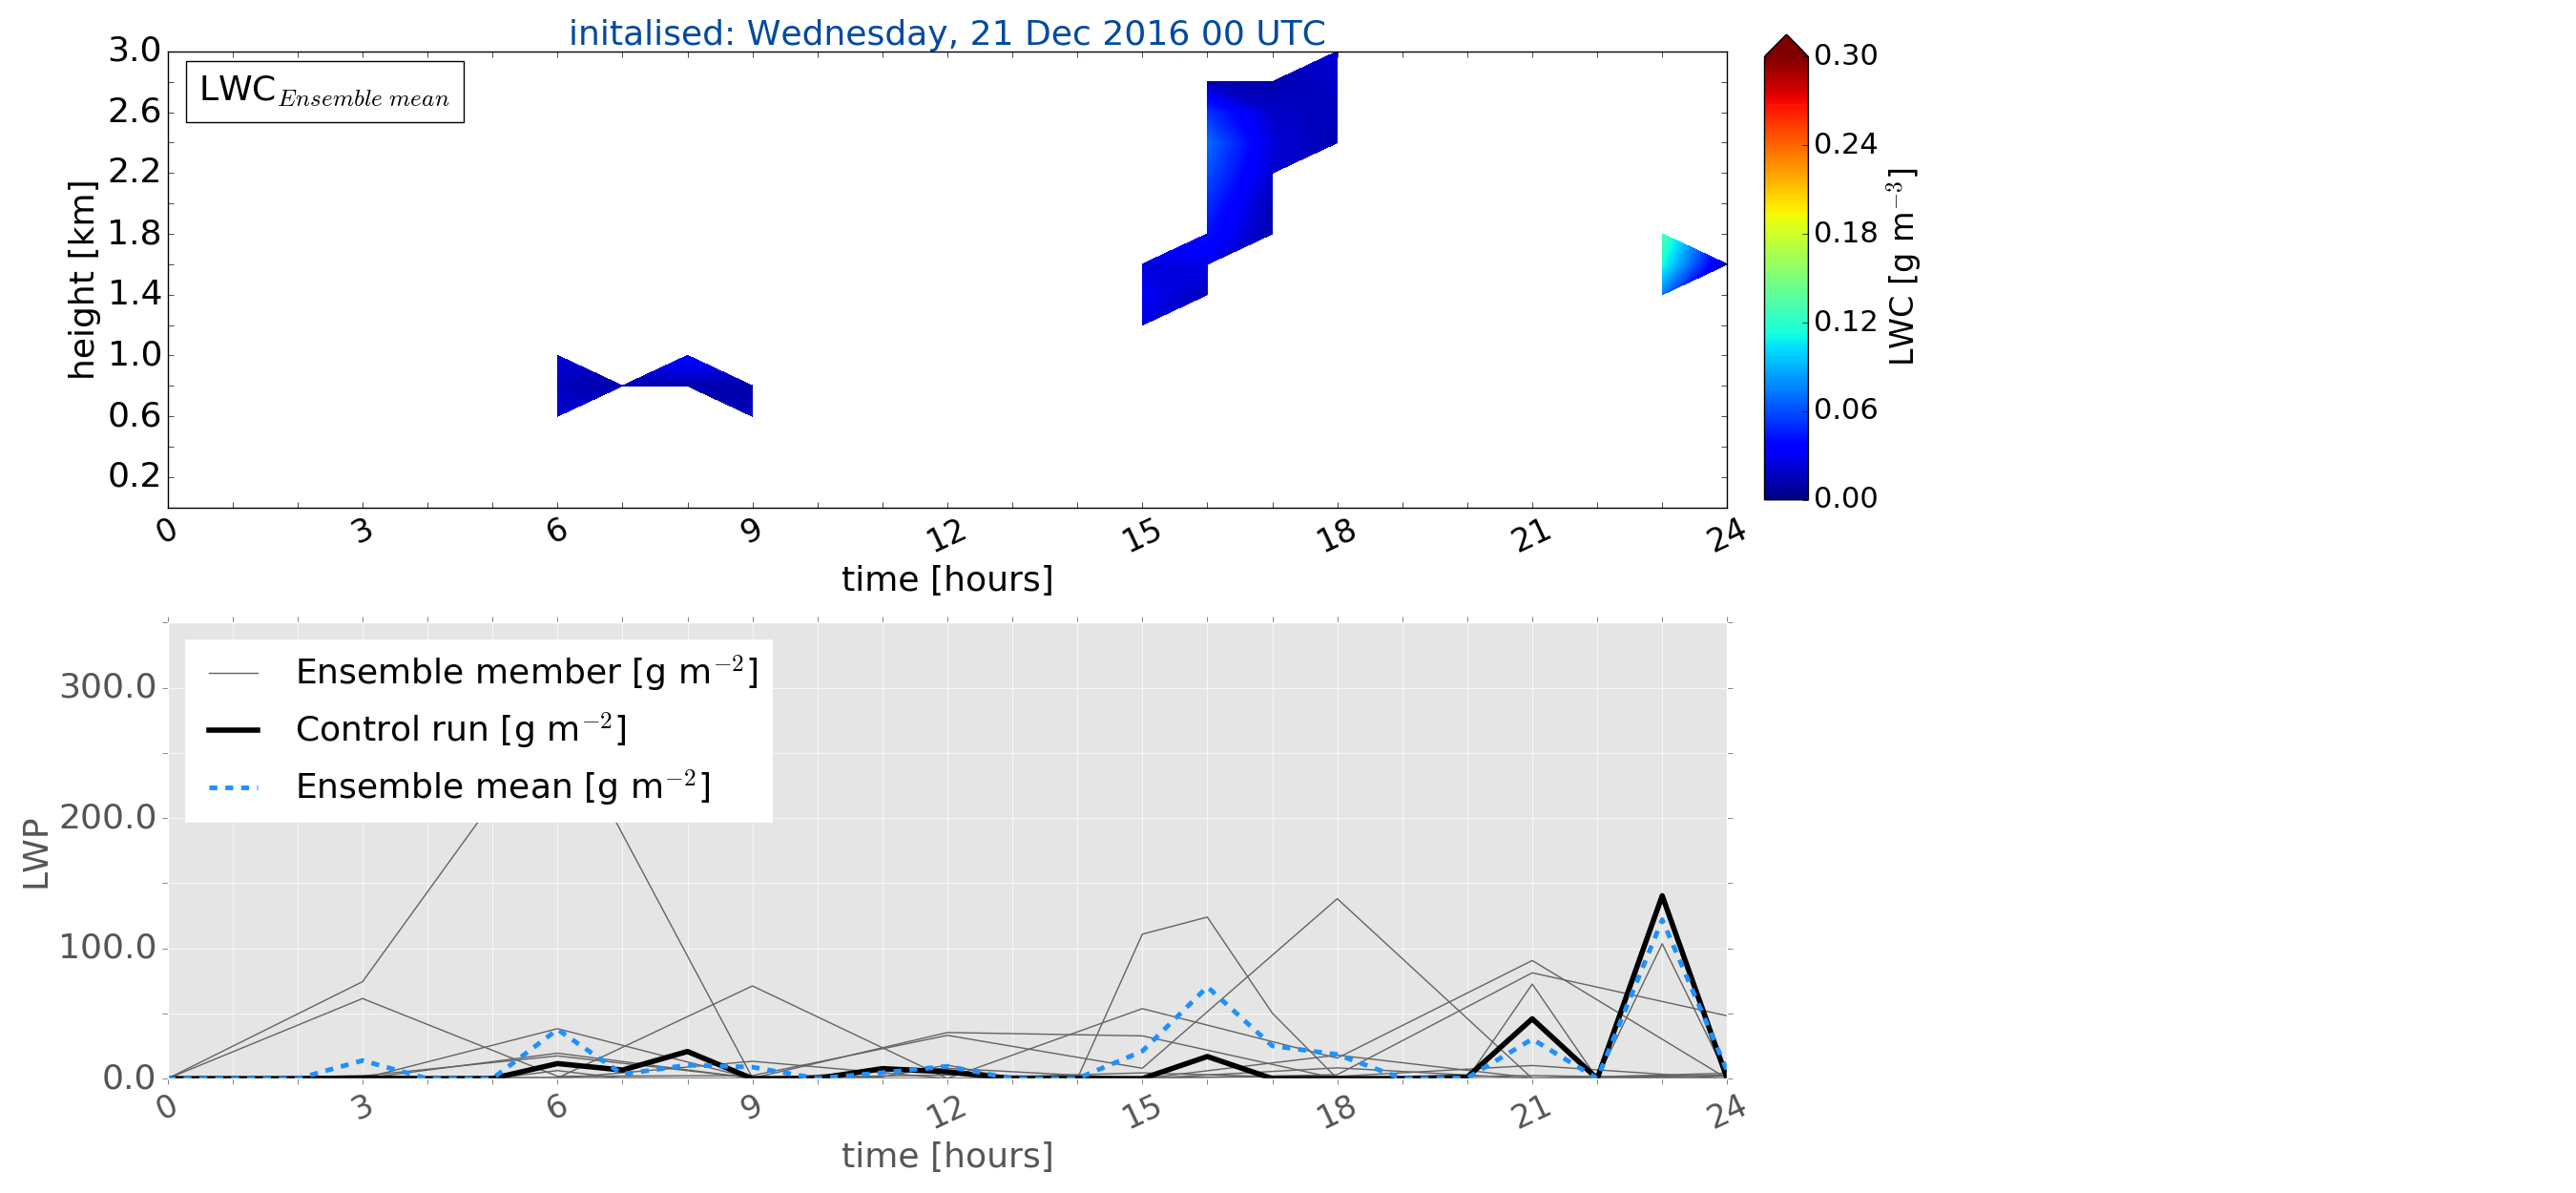
\includegraphics[trim={0.5cm 0.5cm 17.5cm .5cm},clip,width=\textwidth]{./fig_LWC/20161221}
			\caption{}\label{fig:LWC21}
		\end{subfigure}
\end{figure}
\begin{figure}\ContinuedFloat
	\centering
        % 22/12
		\begin{subfigure}[b]{0.8\textwidth}
			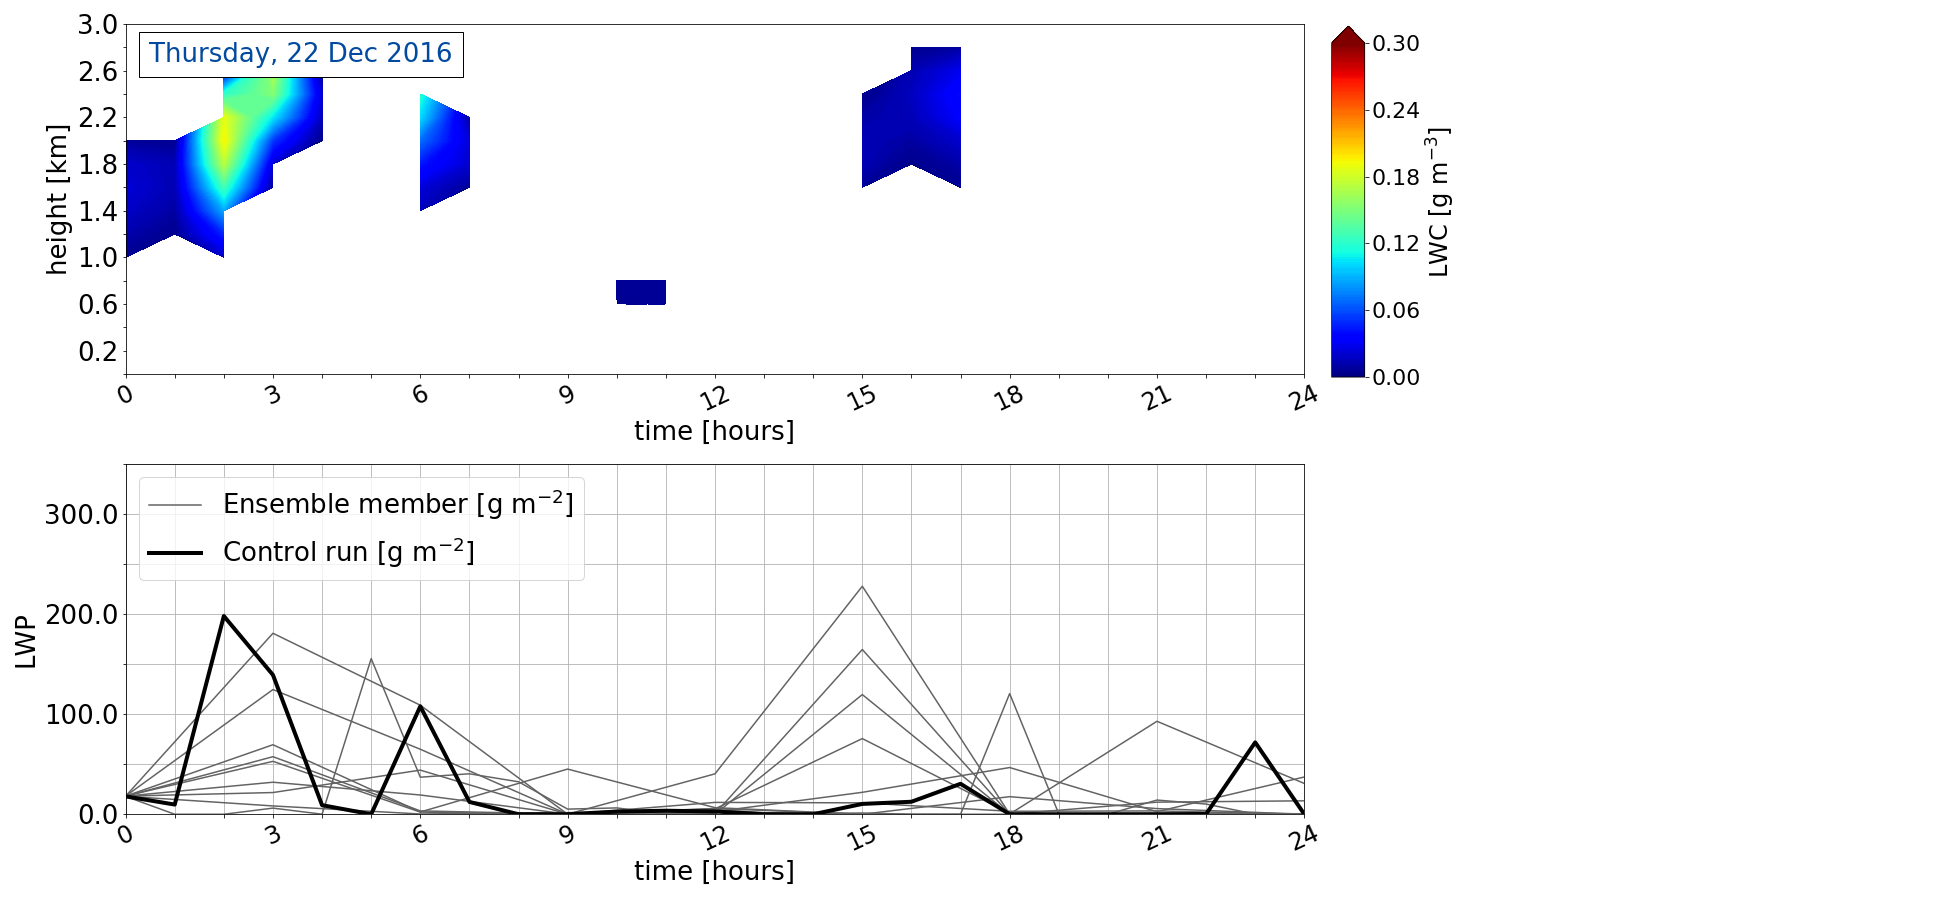
\includegraphics[trim={0.5cm 0.5cm 17.5cm .5cm},clip,width=\textwidth]{./fig_LWC/20161222}
			\caption{}\label{fig:LWC22}
		\end{subfigure}
        % 23/12
		\begin{subfigure}[b]{0.8\textwidth}
			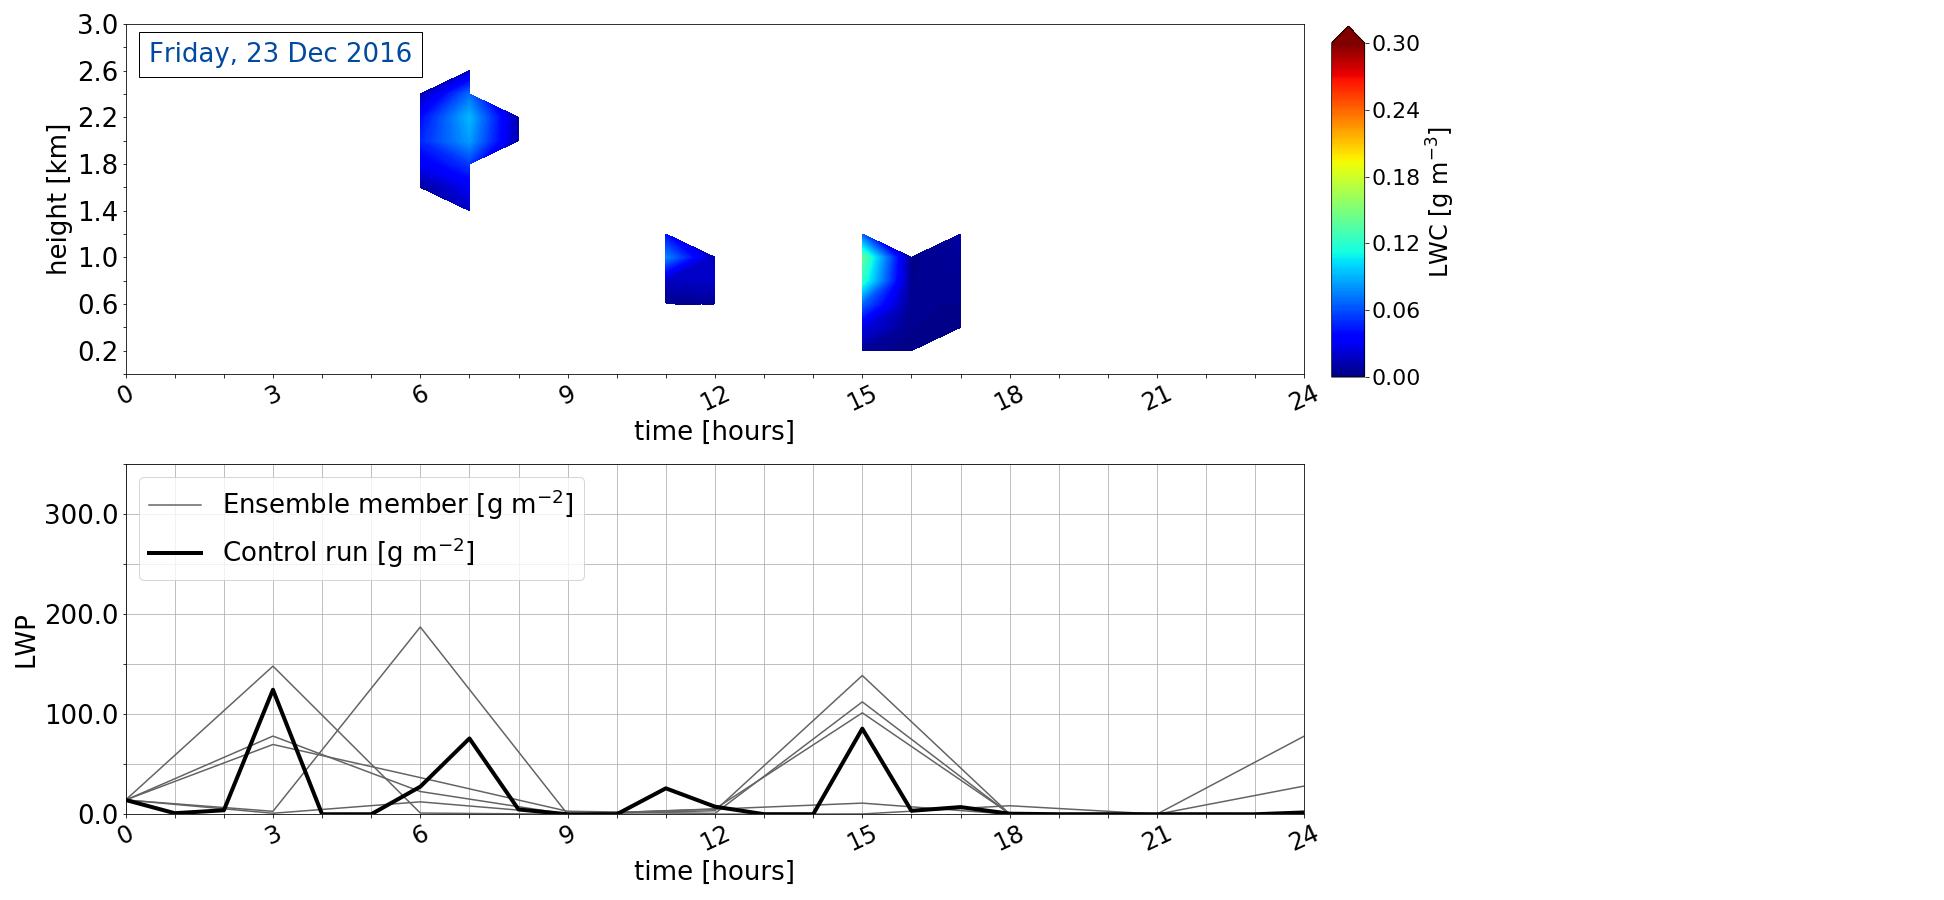
\includegraphics[trim={0.5cm 0.5cm 17.5cm .5cm},clip,width=\textwidth]{./fig_LWC/20161223}
			\caption{}\label{fig:LWC23}
		\end{subfigure}
        % 24/12
		\begin{subfigure}[b]{0.8\textwidth}
			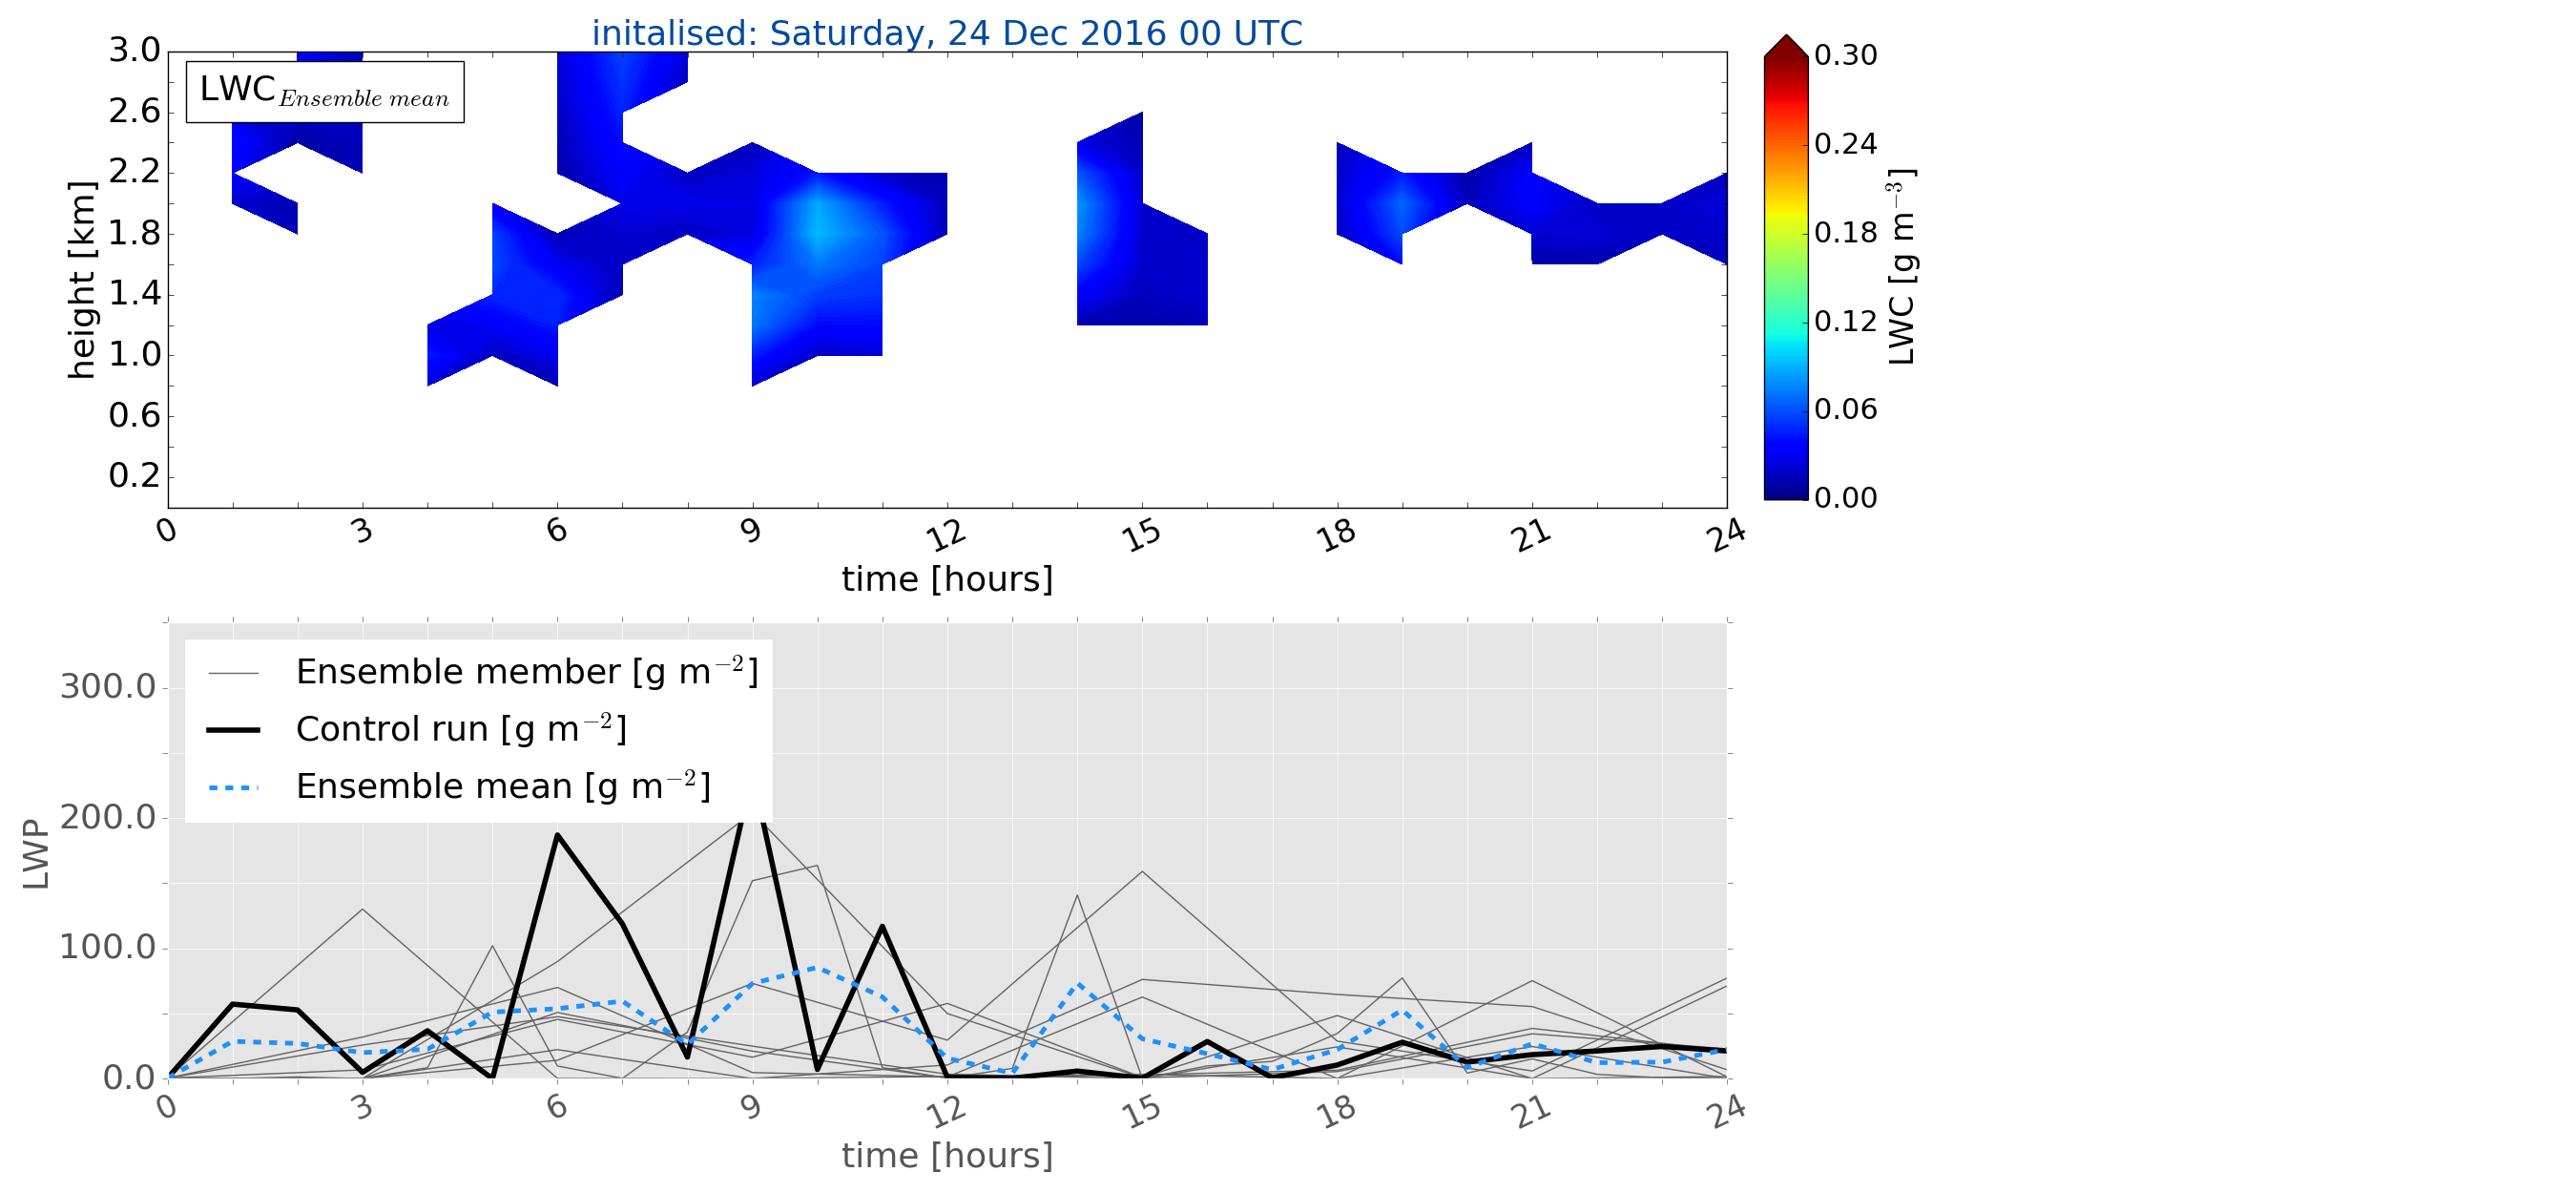
\includegraphics[trim={0.5cm 0.5cm 17.5cm .5cm},clip,width=\textwidth]{./fig_LWC/20161224}
			\caption{}\label{fig:LWC24}
		\end{subfigure}
\end{figure}
\begin{figure}\ContinuedFloat
   		\centering
        % 25/12
		\begin{subfigure}[b]{0.8\textwidth}
			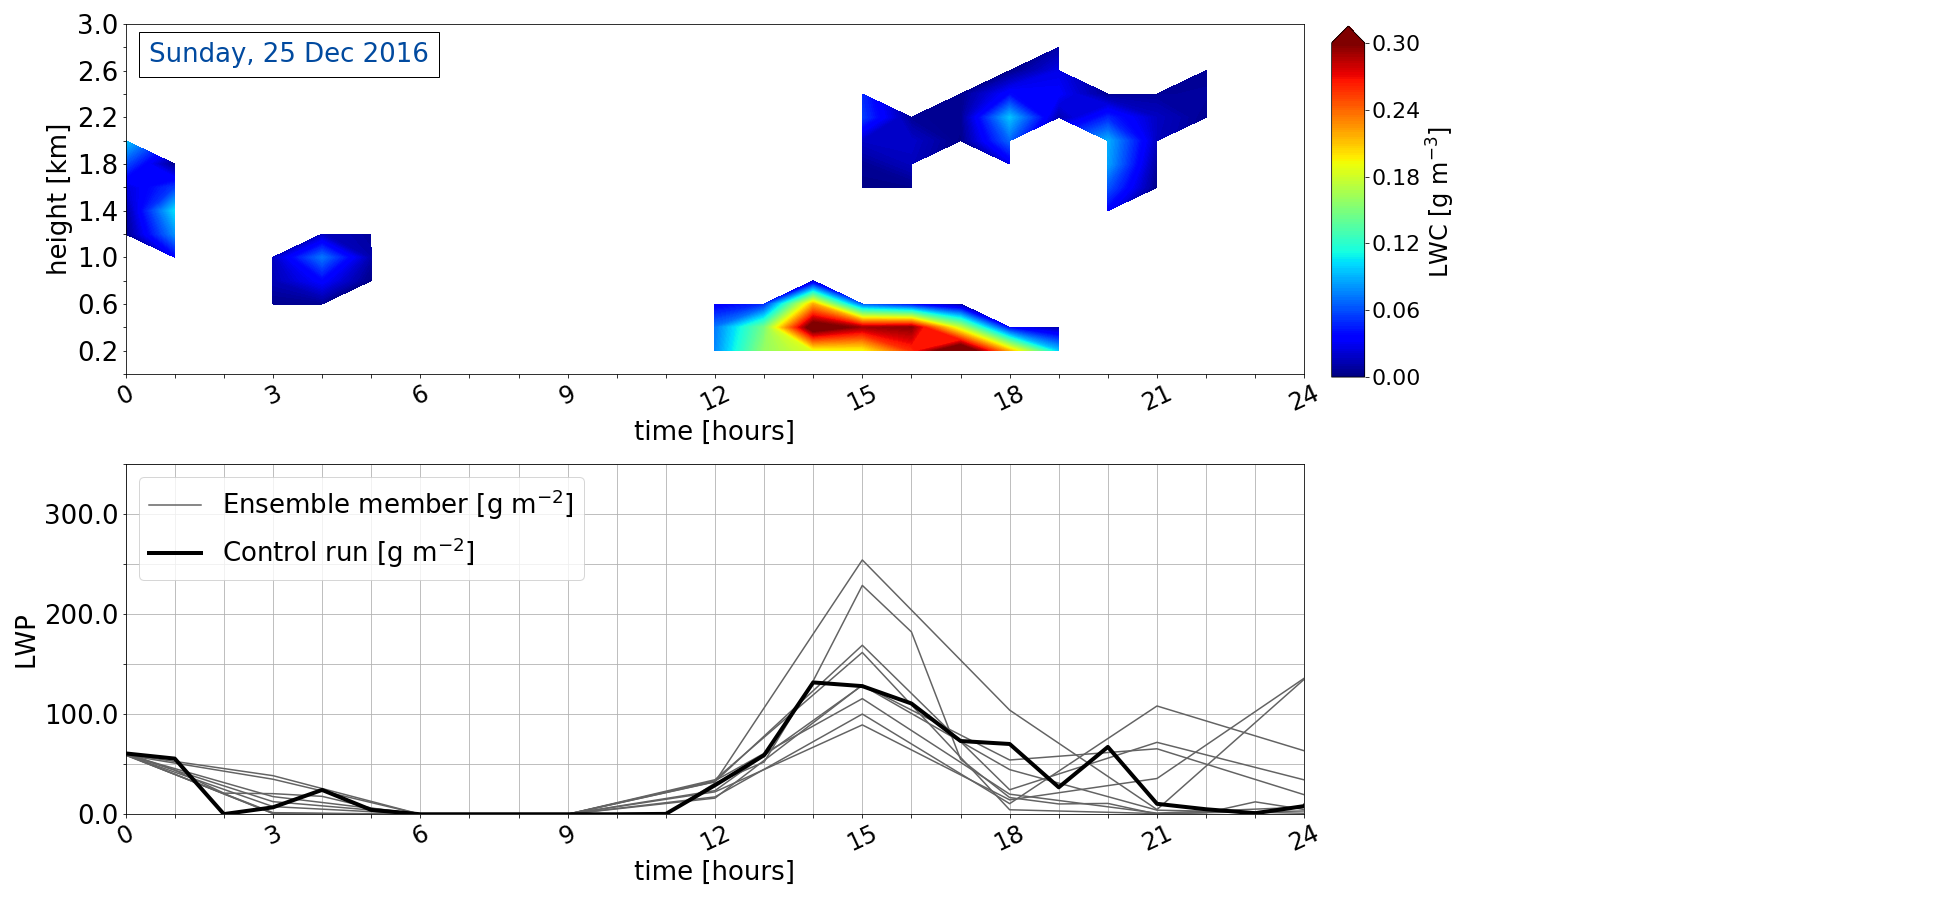
\includegraphics[trim={0.5cm 0.5cm 17.5cm .5cm},clip,width=\textwidth]{./fig_LWC/20161225}
			\caption{}\label{fig:LWC25}
		\end{subfigure}
        % 26/12
		\begin{subfigure}[b]{0.8\textwidth}
			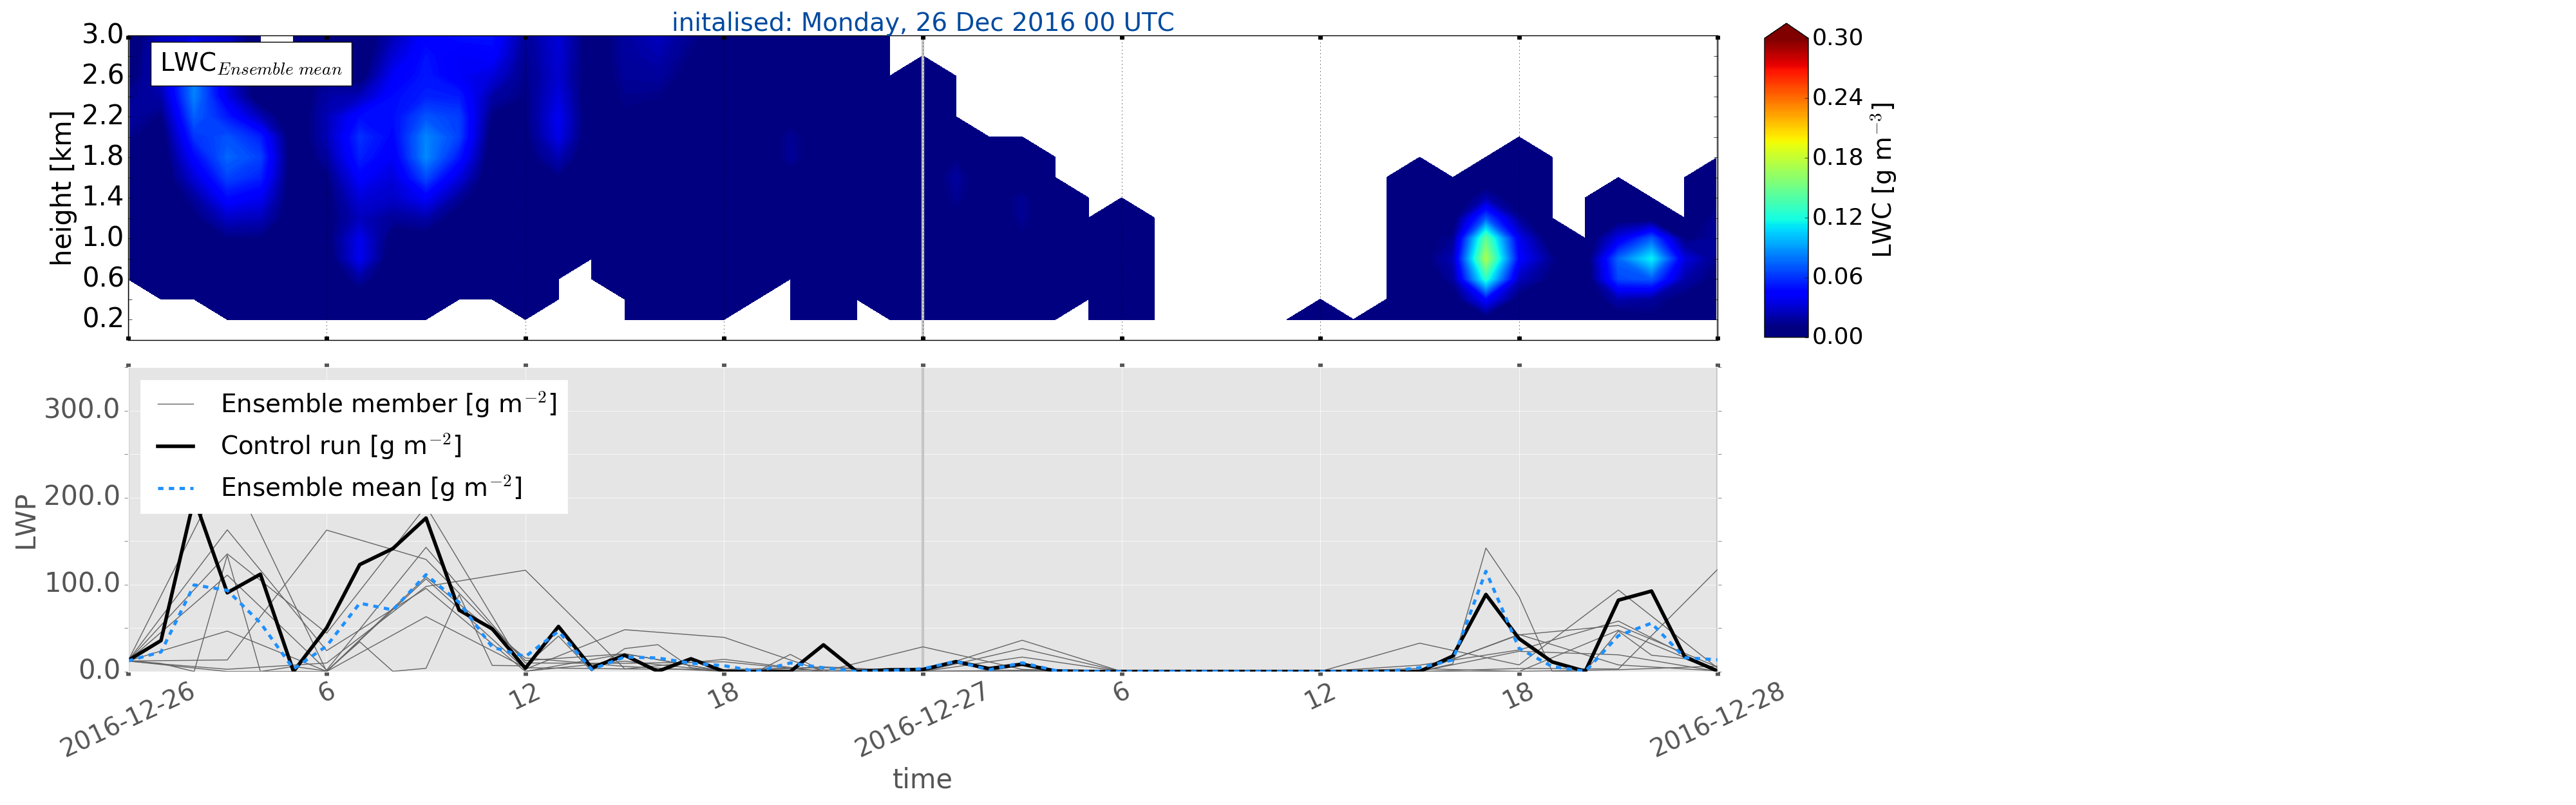
\includegraphics[trim={0.5cm 0.5cm 17.5cm .5cm},clip,width=\textwidth]{./fig_LWC/20161226}
			\caption{}\label{fig:LWC26}
		\end{subfigure}
    \caption{Liquid water content and liquid water path from MEPS.}\label{fig:LWC}
	\end{figure}

	
